
\documentclass[border=5pt]{standalone}
\usepackage{pgfplots}
\pgfplotsset{compat=1.17}
\usepgfplotslibrary{fillbetween}
\begin{document}
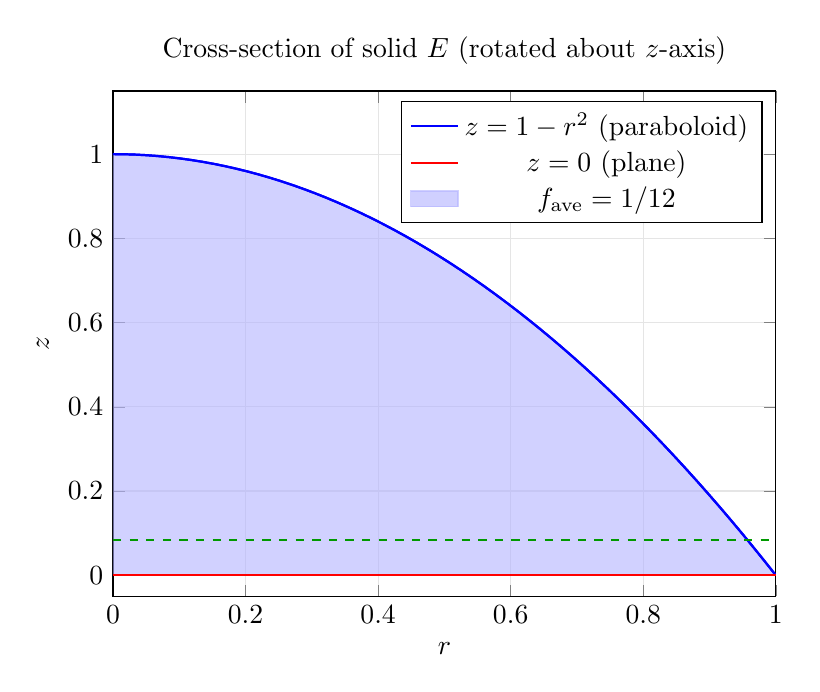
\begin{tikzpicture}
\begin{axis}[
    xlabel={$r$}, ylabel={$z$},
    xmin=0, xmax=1, ymin=-0.05, ymax=1.15,
    width=10cm, height=8cm,
    grid=both, grid style={gray!20},
    title={Cross-section of solid $E$ (rotated about $z$-axis)}]
\addplot[blue, thick, domain=0:1, samples=60, name path=A] {1-x^2};
\addplot[red, thick, domain=0:1, name path=B] {0};
\addplot[blue!30, opacity=0.6] fill between[of=A and B];
\addplot[blue, thick, domain=0:1, samples=60] {1-x^2};
\addlegendentry{$z = 1 - r^2$ (paraboloid)}
\addplot[red, thick, domain=0:1] {0};
\addlegendentry{$z = 0$ (plane)}
\addplot[green!60!black, dashed, thick, domain=0:1] {1/12};
\addlegendentry{$f_{\rm ave} = 1/12$}
\end{axis}
\end{tikzpicture}
\end{document}
